\section{Variant Species}
\DndDropCapLine{V}{}\textbf{ariant Species} are supernatural augmentations laid over a character’s base race, meant to represent curses, blessings, bloodline mutations, divine meddling, magical corruption, or other transformative forces that set an individual apart from ordinary folk.

In most cases, a Variant Species does not replace the traits of the base chosen species, but instead adds new features, modifies existing capabilities, or imposes thematic drawbacks that reflect the nature of the transformation.

\subsection{Dhampir}
Poised between the worlds of the living and the dead, \textbf{dhampirs} retain their grip on life yet are endlessly tested by vicious hungers. Their ties to the undead grant dhampirs a taste of a vampire’s deathless prowess in the form of increased speed (extra 10 m), darkvision, and a life-draining bite. Generally Born of a vampiric woman and a human or dhampir father, these deathless trace their lineage back to the original unnamed Vampire twins; brothers who saught out immortality without the severance of their souls. However rare, dhampir can be created when a human drinks the blood of a vampire and survives. The bite attack starts out with a base damage of \textbf{2d4} that increases to \textbf{2d6, 2d8} and \textbf{2d10} at \textit{levels 4, 8, and 12 respectrively}, that heals the player for the damage dealt.

\subsubsection{Crystalline}
Iridescent and brittle-skinned and incomprehensably beautiful, these dhampir are more durable than their bat-like cousins and generally blend into society better, though crystalline dhampir do not wither beneath the day but instead gleam all the brighter in it, their skin casting prismatic light like living crystal and marking them at once as something not wholly mortal. They gain the \textbf{feat: }\textbf{tough}, but become \textbf{vulnerable to Thunder Damage}.

\subsubsection{Chiropterine}
Bat-like and hairy, though still human-esque in appearance, these dhampir are more animalistic and gain heightened awareness and keen reflexes; marked by its more bestial caste: furred limbs, membranous ears, sharp features, and the restless, twitching alertness of a hunting thing.. They gain the \textbf{dread ambusher feature from Gloomstalker Rangers} but become \textbf{vulnerable to radiant damage}.

\begin{figure}[H]
\centering
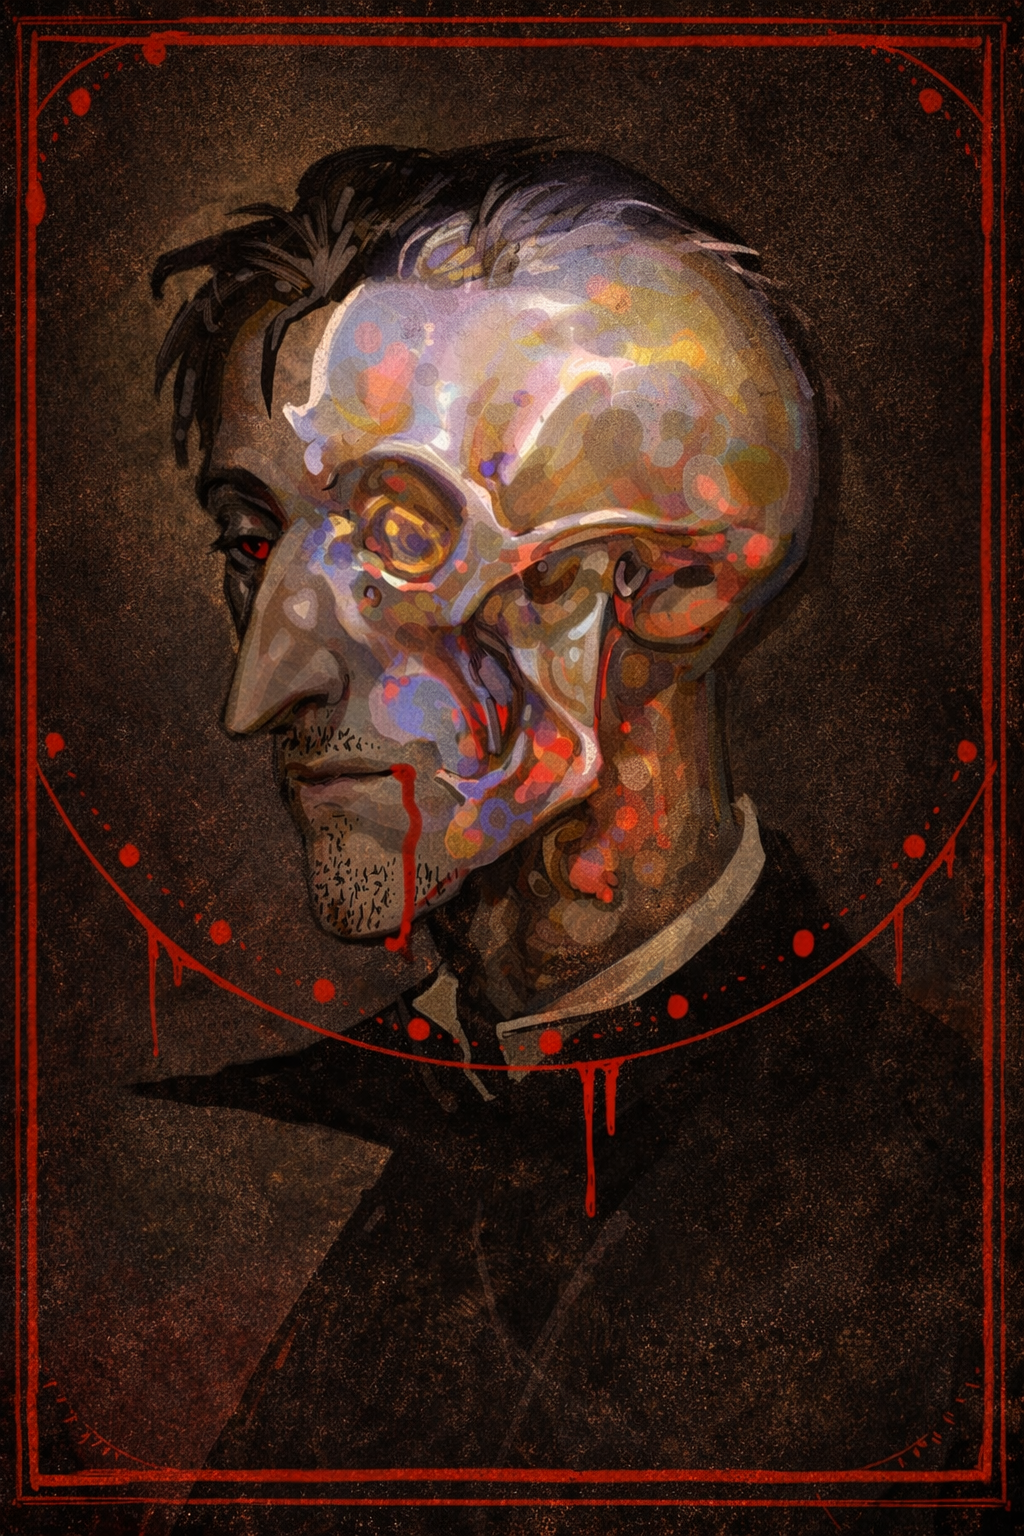
\includegraphics[width=0.225\textwidth]{Images/Dhampir.png}
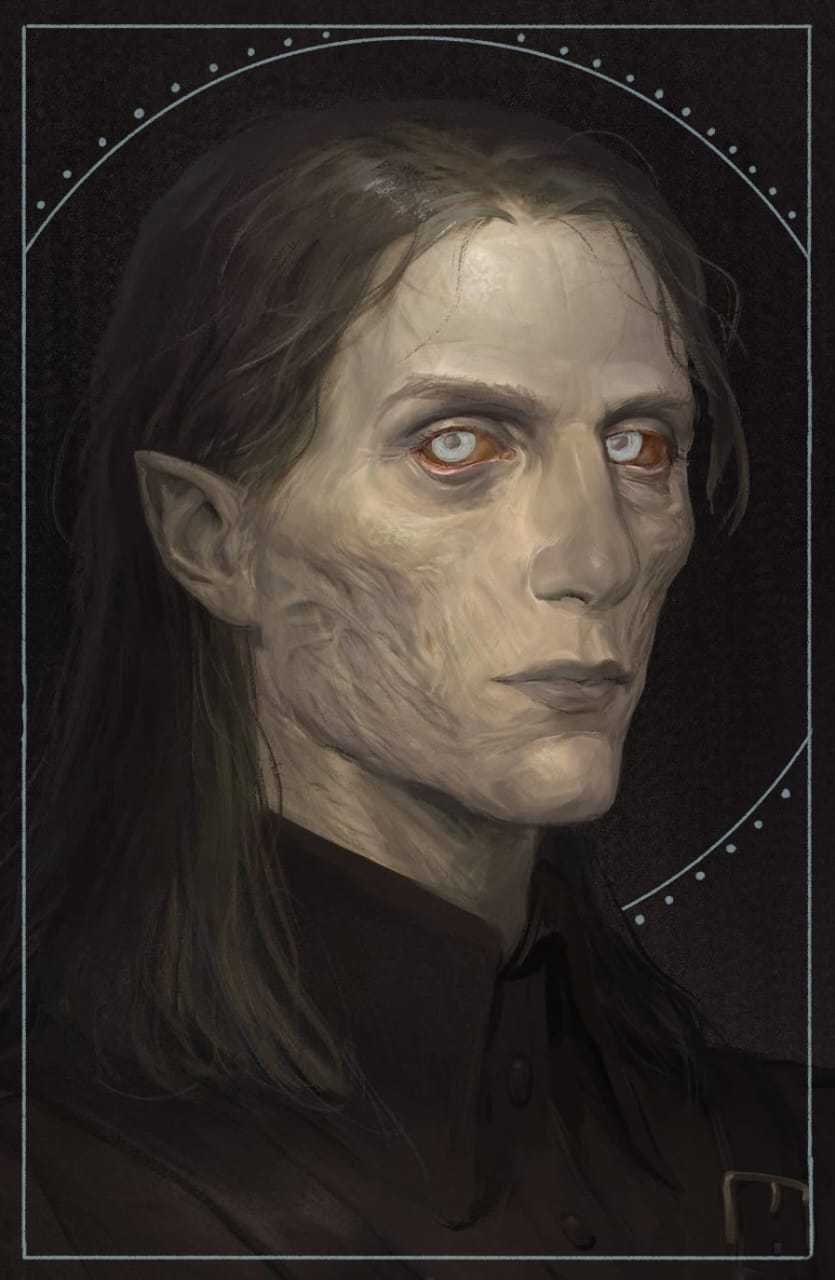
\includegraphics[width=0.22\textwidth]{Images/bat.jpeg}
\end{figure}

\begingroup
\DndSetThemeColor[PhbMauve]
\begin{DndSidebar}{Unholy Offspring}
\textit{The \textbf{Dhampir} are spawned from the cursed womb of a \textbf{Vampiric Matron}, a \textbf{consort to a Vampire Lord}. Often born out of wedlock, bastards to lesser men and dhampir.}
\end{DndSidebar}
\endgroup

\subsection{Chymaera}
The birth of twins aren't uncommon, but the rejoining of the souls within the womb very much is. Through scientific, necromantic or mutagenic interference, these beings born of humans show no physical difference, but harbour two souls. Often frightening parents into thinking their children are schizophrenic or possesed, these misunderstood children often end up lost or killed.
\textbf{Dual Mind. }You have advantage on all Wisdom saving throws.

\textbf{Mental Discipline. }You have resistance to psychic damage.


\textbf{Mind Link. } You can speak telepathically to any creature you can see, provided the creature is within a number of feet of you equal to 10 times your level. You don't need to share a language with the creature for it to understand your telepathic utterances, but the creature must be able to understand at least one language.
       

\textbf{Severed Spirits} Using the power of your other half you can either restore a level 1 spell slot 2 ki points or 1 specialty dice/resource up of a magical nature once every long rest for either yourself or a party member within 30 ft.

\subsection{Reborn}
Death isn’t always the end. The reborn exemplify this, being individuals who have died yet, somehow, still live. Some reborn exhibit the scars of fatal ends, their ashen flesh or bloodless veins making it clear that they’ve been touched by death. Other reborn are marvels of magic or science, being stitched together from disparate beings or bearing mysterious minds in manufactured bodies. Whatever their origins, reborn know a new life and seek experiences and answers all their own.


    \textbf{Ancestral Legacy. }If you replace a race with this lineage, you can keep the following elements of that race: any skill proficiencies you gained from it and any climbing, flying, or swimming speed you gained from it.
        If you don't keep any of those elements or you choose this lineage at character creation, you gain proficiency in two skills of your choice.

    \textbf{Deathless Nature.} You have escaped death, a fact represented by the following benefits:
        You have advantage on saving throws against disease and being poisoned, and you have resistance to poison damage.
        You have advantage on death saving throws.
        You don’t need to eat, drink, or breathe.
        You don’t need to sleep, and magic can’t put you to sleep. You can finish a long rest in 4 hours if you spend those hours in an inactive, motionless state, during which you retain consciousness.



   \textbf{ Knowledge from a Past Life.} You temporarily remember glimpses of the past, perhaps faded memories from ages ago or a previous life. When you make an ability check that uses a skill, you can roll a \textbf{d6} immediately after seeing the number on the \textbf{d20} and add the number on the \textbf{d6} to the check. You can use this feature a number of times equal to your proficiency bonus, and you regain all expended uses when you finish a long rest.

\begin{figure}[ht]
\centering
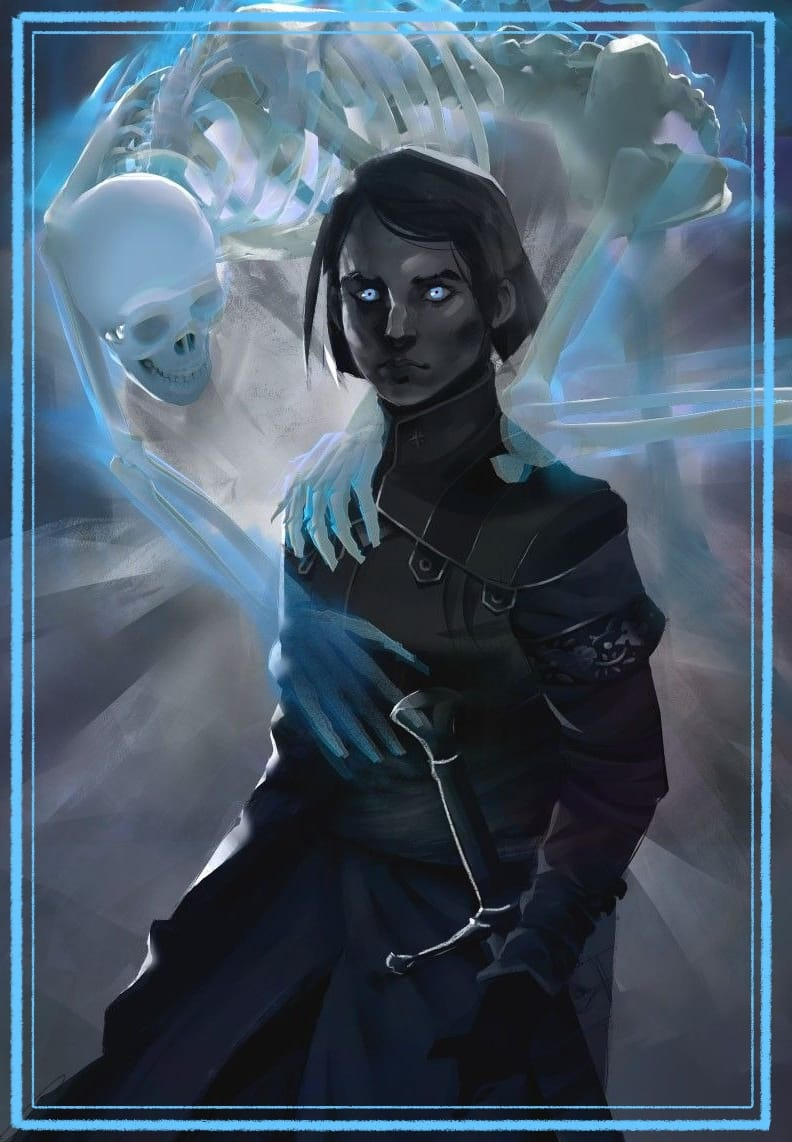
\includegraphics[width=0.228\textwidth]{Images/chym_possible.jpeg}
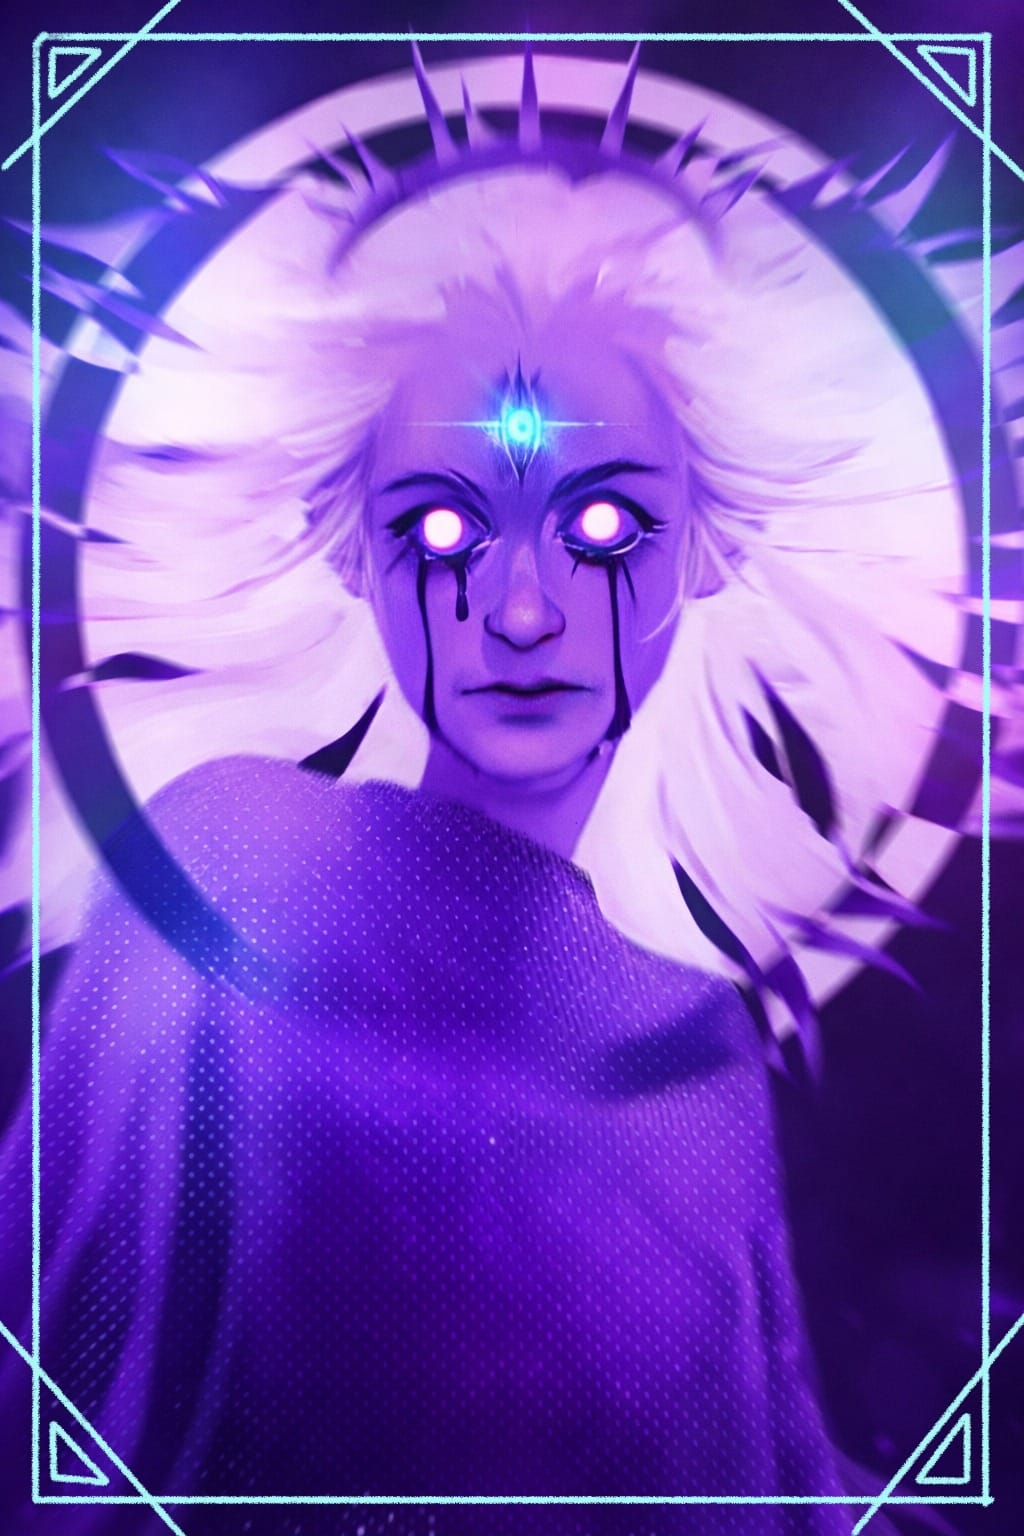
\includegraphics[width=0.22\textwidth]{Images/menari.jpeg}
\end{figure}

\begingroup
\DndSetThemeColor[PhbMauve]
\begin{DndSidebar}{Unholy Offspring}
\textit{The \textbf{Dhampir} are spawned from the cursed womb of a \textbf{Vampiric Matron}, a \textbf{consort to a Vampire Lord}. Often born out of wedlock, bastards to lesser men and dhampir.}
\end{DndSidebar}
\endgroup
